\documentclass[t,aspectratio=169]{beamer} % 使用16:9宽高比
\usetheme{Madrid} % 选择Madrid主题
\usecolortheme{default} % 使用默认颜色主题
\usepackage[UTF8]{ctex}
\usefonttheme{structurebold} % 加粗结构字体
\usepackage{amsmath, amssymb, amsfonts, bm}
\usepackage{url}
\usepackage{graphicx}
% \graphicspath{{./images/}} % 假设图片放在images文件夹

\title[6.2.多层网络]{第6章：深度神经网络}
\subtitle{第2节：多层网络 (Multilayer Networks)}
\author{《深度学习基础》课程小组}
% \institute{上海立信会计金融学院}
\date{\today}

\begin{document}

% 第一张：标题页
\frame{\maketitle}

% 目录页
\begin{frame}
    \frametitle{目录}
    \tableofcontents
\end{frame}

\begin{frame}
\frametitle{多层网络概述}
\begin{itemize}
    \item 对于大规模数据集和高维空间问题，需要找到针对特定问题调整的一组基函数
    \item 神经网络的关键思想是选择具有{\color{red}可学习参数的基函数 $\phi_j(\mathbf{x})$}
    \item 这些参数与系数 $\{w_j\}$ 一起在训练过程中调整
    \item 使用梯度下降法最小化误差函数来优化整个模型
\end{itemize}
\end{frame}

\section{两层神经网络模型}
\begin{frame}
\frametitle{两层神经网络模型（输入层、隐藏层和输出层）}
\begin{itemize}
    \item 构造 $M$ 个输入变量 $x_1, \ldots, x_D$ 的线性组合：
    \(\displaystyle 
    a_j^{(1)} = \sum_{i=1}^{D} w_{ji}^{(1)} x_i + w_{j0}^{(1)}
    \), $j = 1, \ldots, M$.
    \item 每个量 $a_j$ 通过可微非线性激活函数 $h(\cdot)$ 变换：
    \(\displaystyle 
    z_j^{(1)} = h(a_j^{(1)}). 
    \)
\end{itemize}

\begin{figure}
\centering
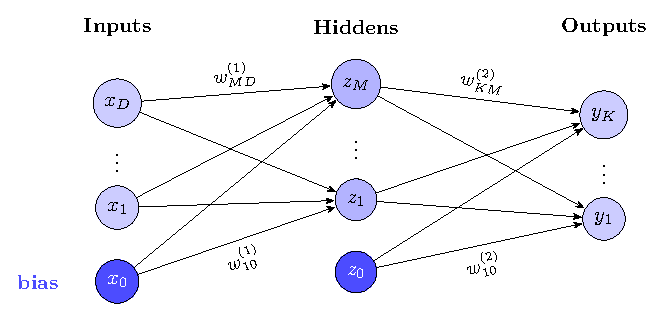
\includegraphics[width=0.6\textwidth]{fig69.pdf}
% \caption{两层神经网络结构：输入层、隐藏层和输出层}
\label{fig:network}
\end{figure}

\end{frame}

\begin{frame}
\frametitle{激活函数}
\begin{itemize}
    \item 这些代表基函数的输出，在神经网络中称为隐藏单元
    \item 最终通过第二层变换得到输出：
    \[
    a_k^{(2)} = \sum_{j=1}^{M} w_{kj}^{(2)} z_j^{(1)} + w_{k0}^{(2)}
    \]
    \item 上标 $(1)$ 表示第一层参数，参数 $w_{ji}^{(1)}$ 称为权重参数，$w_{j0}^{(1)}$ 称为偏置参数
    \item 输出量 $y_k$ 通过可微非线性激活函数 $f(\cdot)$ 变换：
    \[ 
    y_k = f(a_k^{(2)}). 
    \]
\end{itemize}
\end{frame}

\section{参数矩阵}
\begin{frame}
\frametitle{参数矩阵表示}
\begin{itemize}
    \item 偏置参数可以吸收到权重参数中，定义额外输入变量 $x_0 = 1$：
    \[
    a_j = \sum_{i=0}^{D} w_{ji}^{(1)} x_i
    \]
    \item 整体网络函数变为：
    \[
    y_k(\mathbf{x}, \mathbf{w}) = f\left( \sum_{j=0}^{M} w_{kj}^{(2)} h\left( \sum_{i=0}^{D} w_{ji}^{(1)} x_i \right) \right)
    \]
    \item 矩阵形式表示：
    \[
    \mathbf{y}(\mathbf{x}, \mathbf{w}) = f\left( \mathbf{W}^{(2)} h\left( \mathbf{W}^{(1)} \mathbf{x} \right) \right)
    \]
\end{itemize}
\end{frame}

\begin{frame}
\frametitle{通用逼近性质}
\begin{itemize}
    \item 1980年代广泛研究了两层前馈网络的逼近性质
    \item 对于广泛的激活函数，此类网络可以以任意精度逼近 $\mathbb{R}^D$ 连续子集上的任何函数
    \item 类似结果也适用于从任何有限维离散空间到另一个空间的函数
    \item 因此神经网络被称为通用逼近器
\end{itemize}
\end{frame}

\section{隐藏单元激活函数}
\begin{frame}
\frametitle{隐藏单元激活函数}
\begin{itemize}
    \item 隐藏单元激活函数的唯一要求是可微
    \item 最简单的选择是恒等函数，但这等价于无隐藏单元的网络
    \item 常用的非线性可微函数包括：
    \begin{itemize}
        \item Logistic Sigmoid: $\sigma(a) = \frac{1}{1 + \exp(-a)}$
        \item Tanh: $\tanh(a) = \frac{e^a - e^{-a}}{e^a + e^{-a}}$
        \item Softplus: $h(a) = \ln(1 + \exp(a))$
        \item ReLU: $h(a) = \max(0, a)$
    \end{itemize}
\end{itemize}
\end{frame}

\begin{frame}
\frametitle{ReLU及其变体}
\begin{itemize}
    \item ReLU (修正线性单元) 定义为：$h(a) = \max(0, a)$
    \item 经验上表现最好的激活函数之一
    \item 倾斜ReLU (Leaky ReLU) 定义为：
    \[
    h(a) = \max(0, a) + \alpha \min(0, a)
    \]
    \item 其中 $0 < \alpha < 1$
\end{itemize}
\end{frame}

\section{权重空间对称性}
\begin{frame}
\frametitle{权重空间对称性}
\begin{itemize}
    \item 前馈网络的一个特性是多个不同的权重向量 $\mathbf{w}$ 可以产生相同的输入到输出映射
    \item 对于具有 $M$ 个隐藏单元的两层网络：
    \begin{itemize}
        \item 有 $M$ 个"符号翻转"对称性
        \item 有 $M!$ 个交换对称性（对应隐藏单元的不同排序）
        \item 总体对称因子为 $M! 2^M$
    \end{itemize}
\end{itemize}
\end{frame}

\begin{frame}
\frametitle{总结}
\begin{itemize}
    \item 多层网络通过可学习参数的基函数实现复杂模式识别
    \item 两层网络具有通用逼近能力
    \item 不同的激活函数各有优缺点
    \item 权重空间存在对称性，但通常对实际应用影响不大
    \item 深度学习通过更多层实现分层内部表示学习
\end{itemize}
\end{frame}

\end{document}